\chapter[Metodologia]{Metodologia}
\addcontentsline{toc}{section}{Metodologia}

A metodologia que foi escolhida pelo gerente e discutida com todo o grupo foi o SCRUM (Métodos Ágeis). Um dos motivos dessa escolha, em comparação com a metodologia tradicional (PMBoK), é pelo fato do SCRUM ser uma metodologia iterativa e incremental que gera mais resultados em menores ciclos de vidas (sprints). Vale lembrar que o PMBoK (que foca bastante na documentação e no planejamento) é de extrema importância para a manufatura, e o SCRUM para o desenvolvimento de software, ou seja, ambos tem naturezas de projeto diferentes. Para o projeto “Geração de Energia usando Pipas”, o SCRUM tem um papel importante: compartilhar o conhecimento de toda a equipe, discutir os resultados alcançados e não alcançados nas sprints, realizar a retrospectiva das sprints, adaptar as mudanças e acompanhar o progresso e o desenvolvimento do projeto por iterações.

\section{Plano de comunicação}

O plano de comunicação descreve as formas e os meios de comunicação da equipe do projeto “Geração de Energia usando Pipas”, com o objetivo de formalizar o processo de comunicação da equipe, em que esse plano é utilizado por todos os membros do grupo para que cada um possa compreender da mesma forma como se dará a dinâmica de comunicação. Serão descritos as formas de comunicação interna (entre a equipe do projeto) e externa (interessados no projeto), as ferramentas utilizadas e a descrição dos dados dos membros da equipe.

\section{Equipe}

\begin{center}
    \begin{tabular}{| l | l | l |}
    \hline
Nome	&	Função	&	Email para contato	\\ \hline
Henrique Augusto	&	Gerente	&	henriqueaps2003@hotmail.com	\\ \hline
Lucas Matheus	&	Sub-gerente	&	lucasmco@gmail.com	\\ \hline
Ramon Bevilaqua	&	Sub-gerente	&	ramonbev@hotmail.com	\\ \hline
Victor Machado	&	Sub-gerente	&	victor.machado91@gmail.com	\\ \hline
Allan Domingues	&	Membro	&	allandomingues@aluno.unb.br	\\ \hline
Amanda Guimarães	&	Membro	&	amanda.guimaraes15@hotmail.com	\\ \hline
Ariana Flores	&	Membro	&	ariiana.flores@hotmail.com	\\ \hline
Bianca Teixeira	&	Membro	&	biancaffteixeira@hotmail.com	\\ \hline
Daniel Henrique	&	Membro	&	danielhmarinho@gmail.com	\\ \hline
Danovan Martins	&	Membro	&	danovanmartins@hotmail.com	\\ \hline
Davi Dörr	&	Membro	&	davidorr9@hotmail.com	\\ \hline
Davi Pires	&	Membro	&	davidaviaraujo@hotmail.com	\\ \hline
Gustavo Oliveira	&	Membro	&	liveira.gustavo16@gmail.com	\\ \hline
Henrique de Medeiros	&	Membro	&	henrrique_dmg@hotmail.com	\\ \hline
Kleber Brito	&	Membro	&	kleberbritomoreira10@gmail.com	\\ \hline
Leandro Alves	&	Membro	&	leandrosustenido@gmail.com	\\ \hline
Lívia Sant’Anna	&	Membro	&	livia_sant@live.com	\\ \hline
Lucas Raposo	&	Membro	&	lucas.raposo1995@hotmail.com	\\ \hline
Maria Luiza	&	Membro	&	lulutupy@hotmail.com	\\ \hline
Matheus Bolelli	&	Membro	&	bolellib13@hotmail.com	\\ \hline
Pedro Filhusi	&	Membro	&	pedro_filhusi@hotmail.com	\\ \hline
Rafael Freitas	&	Membro	&	rafa.farias@hotmail.com	\\ \hline
Samuel Medeiros	&	Membro	&	samuelmedeiros.csilva@gmail.com	\\ \hline
Vladimir Nogueira	&	Membro	&	vladifn@gmail.com	\\

    \hline
    \end{tabular}
\end{center}

\section{Comunicação Interna}

A comunicação interna descreve as formas de comunicação entre toda a equipe do Projeto Integrador de Engenharia 1, com o gerente, subgerentes e todos os membros da equipe. Através da tabela abaixo, será descrito o meio de comunicação e local, a data e os horários das reuniões, em que todas as reuniões serão realizadas semanalmente.

\begin{center}
    \begin{tabular}{| l | l | l | l |}
    \hline
Equipes Envolvidas	&	Horário	&	Dias	&	Meio de Comunicação e Local	\\ \hline
Grupo 3 - PI 1	&	16:00 - 18:00	&	Segunda	&	Presencial (FGA) - Sala i9	\\ \hline
Grupo 3 - PI 1	&	16:00 - 18:00	&	Quarta	&	Presencial (FGA) - Sala i4	\\

    \hline
    \end{tabular}
\end{center}

\section{Comunicação Externa}

A comunicação externa se refere aos interessados no projeto que não estão envolvidos diretamente em sua construção. O meio de comunicação que será utilizado no projeto para a comunicação externa será o SCRUMME, onde serão disponibilizados todas as histórias de usuário com as respectivas atividades e pessoas responsáveis da EAP produzidos para os interessados (externos a equipe) no projeto acompanhar o progresso e o desenvolvimento dos mesmos.

\section{Ferramentas}

A tabela a seguir descreve todas as ferramentas utilizadas na comunicação tanto interna quanto externa do projeto. Através da tabela, é descrito o nome da ferramenta e uma breve descrição dela.

\begin{center}
    \begin{tabular}{| l | l |}
    \hline
Ferramentas & Descrição \\ \hline
Facebook & Ferramenta para avisos e interação entre os membros da equipe	\\ \hline
WhatsApp & Aplicativo para celular que permite uma rápida comunicação
e avisos urgentes entre a equipe	\\ \hline
Google Drive & Ferramenta para armazenamento e compartilhamento de
 documentos do projeto \\
    \hline
    \end{tabular}
\end{center}

\section{Ferramentas de gerenciamento}

A ferramenta de gerenciamento de projeto escolhida pelo gerente foi o SCRUMME, pois ele aborda e resume todos os conceitos da Metodologia de Gerenciamento de Projeto SCRUM (Métodos Ágeis). Nessa ferramenta, é possível ver todas as sprints (como gráfico de Burndown e estatísticas da sprint, para analisar o progresso e o desenvolvimento das atividades e da análise de cada pessoa responsável pelas atividades) e suas respectivas histórias de usuário e pessoas relacionadas em cada atividade da EAP (Estrutura Analítica de Projeto). Ela é bastante organizada e interativa, em que isso facilita muito a comunicação com o cliente (patrocinador) do nosos projeto.

\begin{figure}[p]
    \centering
    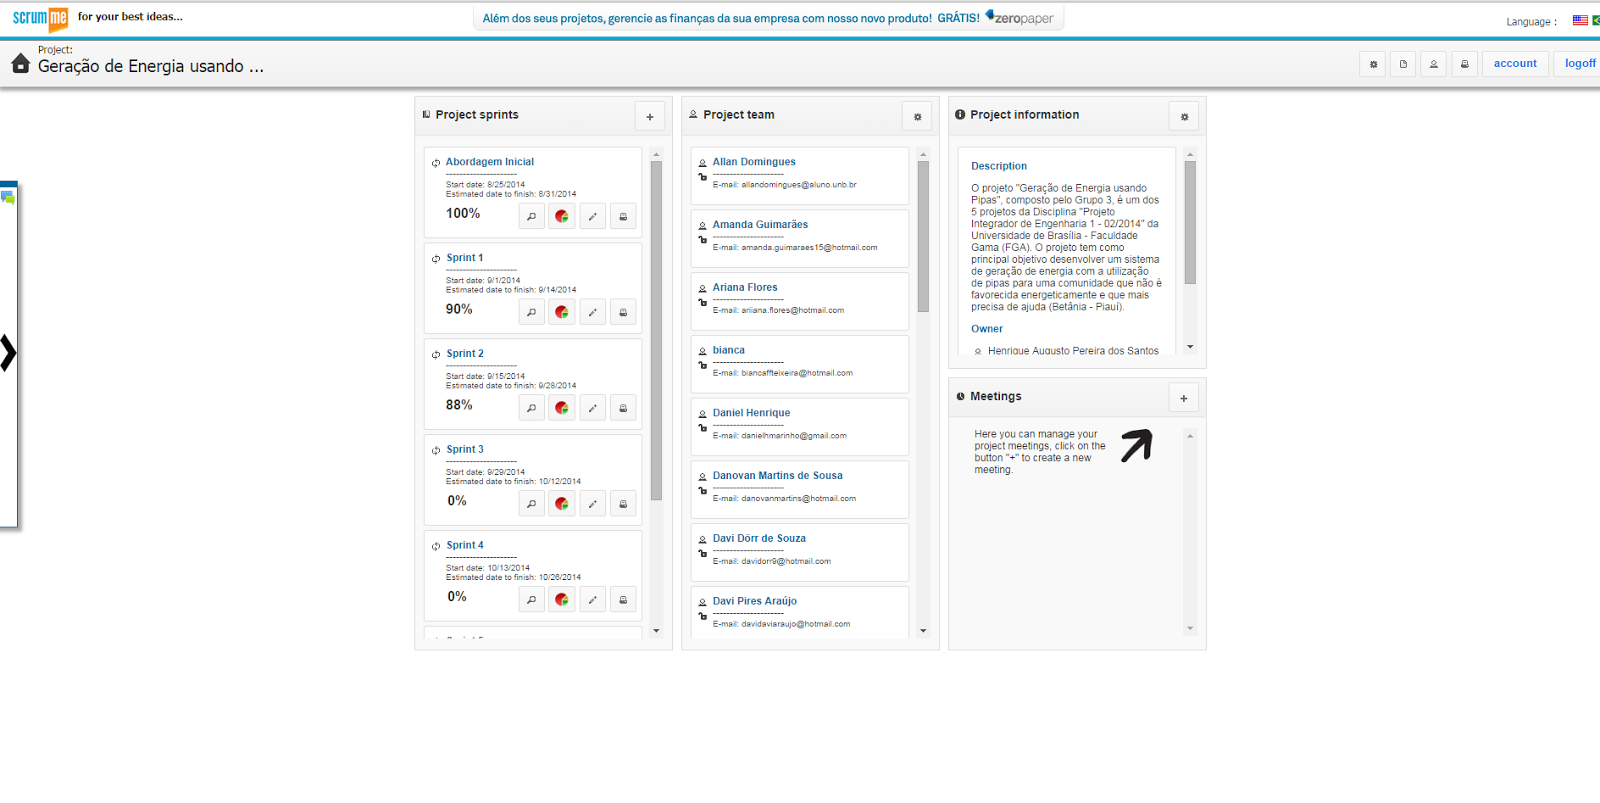
\includegraphics[width=0.8\textwidth]{figuras/scrumme1.png}
    \caption{SCRUMME}
    \label{fig:scrumme}
\end{figure} 